\documentclass{beamer}

\usepackage{gensymb}
\usepackage[utf8]{inputenc}
\DeclareUnicodeCharacter{00A0}{ }%Permet d'éviter certains conflits de caractères invisibles
\usepackage{amssymb}            % Principaux symboles
%\usepackage{fontspec}
%\usepackage{xunicode}
%\usepackage{xltxtra}
\usepackage[frenchb]{babel}
%\defaultfontfeatures{Scale=MatchLowercase}
%\setmainfont[Mapping=tex-text,Ligatures={Common, Historical}]{Linux Libertine O}
%\setsansfont[Mapping=tex-text]{Linux Biolinum O}
%\setmonofont[Scale=0.75]{DejaVu Sans Mono}

%% Packages pour le texte
%\usepackage[misc,geometry]{ifsym}	% Police numéros battons
\usepackage{pifont}		% Police \ding
\usepackage{eurosym}		% Symbole de l'euro
\usepackage{soul}		% Souligner
\usepackage{enumerate}		% Listes
\usepackage{verbatim}		% Codes source
\usepackage{moreverb}		%	et listings
\usepackage{textcomp}
\usepackage{multicol}

%% Packages pour les tableaux
\usepackage{array}		% Outils supplémentaires
\usepackage{multirow}		% Colonnes multiples
\usepackage{tabularx}		% Largeur totale donnée
\usepackage{longtable}		% Sur plusieurs pages

%% Les packages pour les dessins
\usepackage{graphicx}		% Insertion de figures
%\usepackage{picins}		% Dans un paragraphe
\usepackage{epic}		% Capacités graphiques
\usepackage{eepic}		% 	étendues
\usepackage{afterpage}		% Voir page 69
\usepackage{rotating}		% Tourner du texte
\usepackage{caption}		% Légendes
% \addto\captionsfrench{\def\figurename{}}

%% Packages pour les maths
\usepackage{amsmath}		% Commandes essentielles
\usepackage{amssymb}		% Principaux symboles
\usepackage{mathrsfs}		% Police calligraphique
\usepackage{theorem}		% Théorèmes
%\usepackage{tikz}		% Courbes
\usepackage{esvect}            % Vecteurs
%\usetikzlibrary{shapes,arrows,shadows}
\usepackage{pgf}
%\usetikzlibrary{arrows}
% Packages pour la physique
%\usepackage{sistyle}		% Unités
\usepackage[version=3]{mhchem}	% Formules chimiques
\usepackage{etex}
%\usepackage{m-pictex,m-ch-en}

%\usepackage{media9}
\usepackage{multimedia}		% Vidéos dans la présentation
%\usepackage{movie15}

%Ajout d'images de fond:
\usepackage{eso-pic}
\usepackage{wallpaper}

\usepackage{ccicons}		% Licence creativecommons

%\SIdecimalsign{,}


\AtBeginSection[]
{
  \begin{frame}
    \frametitle{Sommaire}
    \begin{multicols}{2}
      {\small
				\setcounter{tocdepth}{2}
        \tableofcontents[currentsection, hideothersubsections]}
    \end{multicols}
  \end{frame}
}

\usetheme{Warsaw}

\usepackage{listings}
\usepackage[babel=true]{csquotes}
\lstset{language=Python, tabsize=2, breaklines=true, showstringspaces=false}

\useoutertheme{infolines}
\setbeamersize{text margin left=1cm,text margin right=1cm}

\title{Rapport de projet de SI}
\subtitle{Tropodrone}
\author{Gueydan Noé, Manceau Thibaut, Gros Alexis, Porteries Tristan}

\begin{document}

\begin{frame}
  \titlepage
\end{frame}

\begin{frame}
    \frametitle{Sommaire}
    \begin{multicols}{2}
      {
		\setcounter{tocdepth}{1}
        \tableofcontents
      }
    \end{multicols}
\end{frame}

\section{Courte présentation}

\subsection{But du projet}

\begin{frame}
 Créer une structure composée de ballons contenant un gaz plus léger que l’air qui soutient une partie ou la totalité du poids d'un drone.
\end{frame}


\subsection{Objectifs}

\begin{frame}
 Augmenter l’autonomie, la sécurité et les possibilités d’un drone de petite taille
\end{frame}


\subsection{Contraintes imposées au projet}
\begin{frame}
  \begin{itemize}
    \item Être simple d’utilisation, garder la manœuvrabilité du drone au possible, voler le plus longtemps possible.
    \item Consommer le moins d’énergie possible, ne pas présenter de danger pour le public et économiser le gaz et les matériaux de fabrication.
    \item Le modèle du drone imposé
    \item Rayon d’action de minimum 15 mètres
    \item Ballon de type dirigeable
  \end{itemize}
\end{frame}

\subsection{Contraintes légales supplémentaires}
\begin{frame}
  \begin{itemize}
    \item 1: Le drone \\
	    Catégorie A : limitations non contraignantes
    \item 2: Le ballon \\
	    Catégorie « Léger » \\
	    La ficelle supportant la charge doit casser au dessus de 23 kg
 \end{itemize}
\end{frame}


\section{Structure}

\subsection{Gyroscope et axes}

\begin{frame}
  
\end{frame}

\subsection{Attaches et modélisation}

\section{Ballon}

\subsection{Contenance}

\subsection{Forme}

\begin{frame}
  Les ballon sont formés d'un parallèlépipède avec deux pyramides d'angle $60\degree$. \\
  \begin{center}
    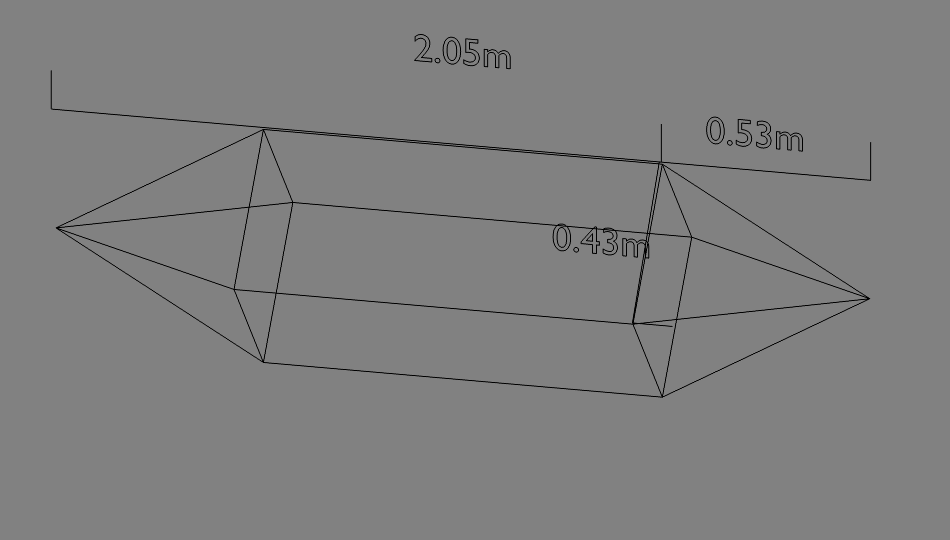
\includegraphics[width=10cm]{../Images/ballon.png}
  \end{center}
\end{frame}

\begin{frame}{Calcul des dimensions}
  Volume ballon~:
  \begin{center}
    $\displaystyle{V = b^3 \sin \frac{\pi}{3} \times \frac{1}{3} + b^2}$ \\
    $\displaystyle{V = b^3 \frac{\sqrt{3}}{6} + b^2}$ \\
    $\displaystyle{b^3 \frac{\sqrt{3}}{6} + b^2 - 0.25 = 0}$
  \end{center}
  Polynome du troisième degrée, résolution par bissection ou dichotomie.
\end{frame}

\begin{frame}[fragile]{Résolution par bissection}
  \begin{lstlisting}[frame=single]
etape = 1
largeur = 1
vol = volume(largeur)
cible = 0.25
epsilon = 1e-4
while abs(vol - cible) > epsilon:
	if vol < cible:
		largeur += etape
	else:
		largeur -= etape
	etape /= 2
	vol = volume(largeur)

print("volume = %f, diametre = %f" % (vol, largeur))
  \end{lstlisting}
\end{frame}

\subsection{Enveloppe}

\begin{frame}
  \begin{multicols}{2}
    \begin{itemize}
      \item Latex~:
      \begin{itemize}
        \item Facile à trouver dans le commerce,
        \item Seulement en forme sphèrique,
        \item Peu étanche~;
      \end{itemize}
      \item Chloroprène~:
      \begin{itemize}
        \item Introuvable dans le commerce~;
      \end{itemize}
      \item Butyle~:
      \begin{itemize}
        \item Introuvable dans le commerce~;
      \end{itemize}
    \end{itemize}
    \newpage
    \begin{itemize}
      \item Mylar~:
      \begin{itemize}
        \item Facile à trouver dans le commerce~;
        \item Resistant à la traction~;
        \item Peu être assembler~;
        \item Raide~;
        \item Fragile au cisaillement.
      \end{itemize}
    \end{itemize}
  \end{multicols}
\end{frame}

\subsection{Collage}

\begin{frame}
  \begin{itemize}
    \item Néoprène(Polychloroprène)
    \begin{itemize}
      \item Etanche
      \item Elastique
      \item Adhèrent
      \item Difficile à appliquer
    \end{itemize}
    \item 406(colle) et 770(primaire)
    \begin{itemize}
      \item Adhèrent
      \item Rigide
      \item Difficile à appliquer
    \end{itemize}
  \end{itemize}
\end{frame}

\subsection{Gonflage}

\section{Calculs d'élévation}

\subsection{Poussé d'archimède}

\begin{frame}{Définition}
  \enquote{Tout corps plongé dans un fluide au repos, entièrement mouillé par celui-ci ou traversant sa surface libre, subit une force verticale, dirigée de bas en haut et opposée au poids du volume de fluide déplacé ; cette force est appelée poussée d'Archimède.}
  \bigbreak
  \begin{center}
    $\vv{P_A} = -M_F \times \vv{g}$
  \end{center}
  $\vv{P_A}$~: La poussé d'archimède. $M_F$ La masse du fluide contenue dans le volume déplacé. $\vv{g}$ La valeur du champ de pesanteur.
\end{frame}

\begin{frame}{Aplication aux gaz}
  Deux forces appliquées sur le ballon~: \\
  \begin{center}
    $\displaystyle{\vv{F_{ballon}} = \vv{P_{ballon}} + \vv{P_{A_{ballon}}}}$ \\
  \end{center}
  Si $P_{ballon} < P_{A_{ballon}}$ la force d'élévation est~:
  \begin{center}
    $\displaystyle{F_{ballon} = P_{A_{ballon}} - P_{ballon}}$ \\
  \end{center}
  Remarque~:\\
  \begin{center}
    $F_{ballon} < P_{A_{ballon}}$
  \end{center}
\end{frame}

\subsection{Dilatation des gaz}

\begin{frame}{Loi de Charles}
  \begin{center}
    $\displaystyle{\frac{V_1}{T_1} = \frac{V_2}{T_2} = f(P, n)}$
    $\displaystyle{V_3 = f(P, n) \times T_3}$
  \end{center}
  $V_q$~: volume du gaz à la température $T_q$. $P$~: pression du gaz. $n$~: quantité de matière. $f(P, n)$~: rapport constant entre volume et température.
\end{frame}

\begin{frame}{Application à l'hélium}
  Volume molaire de l'hélium~: $22.414\times 10^{-3} m^3.mol^{-1}$ à $273.25K$.
  \begin{center}
    $\displaystyle{f(P, n) = \frac{22.414\times 10^{-3}}{273.25} = 8.2\times 10^{-5} m^3.mol^{-1}.K^{-1}}$
  \end{center}
  Pour $T_{200} = 200 \degree C = 473.25 K$~:
  \begin{center}
    $\displaystyle{V_{T_{200}} = 8.2\times 10^{-5} * 473.25 = 38.811 \times 10^{-3}}$
  \end{center}
  Augmentation du volume de $1.59$.
\end{frame}

\begin{frame}{Résultat de la poussé d'archimède}
  \begin{center}
    $\displaystyle{F_{T_0} = P_{air} - P_{helium} = 10.90 N}$
    \bigbreak
    $\displaystyle{F_{T_{200}} = P_{air} - \frac{P_{helium}}{1.59} = 11.57 N}$ \\
  \end{center}
  Les resultats sont négligables. $F < P_{air}$
\end{frame}

\section{Drone}

\subsection{Modèle}

\begin{frame}
  \begin{itemize}
    \item Le dronne est un xcsource (XCSOURCE® Fibre de Carbone Mini 250 FPV Quadcopter ) dont les plant sont en licence libre et notre modek obtenus auprès du fabricant officiel.

    \item Il est fournis d’un chassie en carbone de dimention : 290mm de diagonale , 190 mm de long et 70mm de haut. Ce chassie et a deux nivaux pour faciliter l’ajout des différant composant de vol.

    \item Les moteurs fournis sont des EMAX MT2204 2300KV Brushless Motor. Ils sont alimenter en courant triphasée.Il consomment au maximum en 12v  11,5 A soit 138w. Cette puissance est nécessaire pour faire décoller le drone , le maintenir face a des vents violent ou lui permettre de porter de lourde charge . c’est aussi cette puissance qui limite l’autonomie. Le kit en contiens 4 , 2 tournant en sens trigonométrique et deux tournant en sens anti-trigonométrique

    \item La batterie que nous nous sommes procurés est une Accu Lipo Gens Ace 2200Mah 11.1V 25C 3S. Elle fournie donc 11,1 volt  plainne charge , est composé de 3 cllule de lithium polymere et peux délivrer au maximun
  \end{itemize}
\end{frame}

\subsection{Capacité et poids}

\section{Aérodynamisme}

\subsection{Équation de traînée}
\begin{frame}{Équation de traînée}
 But : que le drone soit le moins sensible à l'air possible \\
 Force de traînée matérialisée par l'équation \\
 \begin{center}
  $\displaystyle{\frac12 \rho S Cx V^2}$
 \end{center}
\end{frame}

\subsection{Calcul de Cx pour la forme retenue 1/2}
\begin{frame}{Calcul de Cx pour la forme retenue 1/2}
 Forme la plus proche : sphère \\
 Dépend du type d'écoulement : le nombre de reynolds \\
 \begin{center}
  $\begin{array}{>{\displaystyle}l>{\displaystyle}l>{\displaystyle}l}
   Re < 1 & Cx = & \frac{24}{Re} \medbreak \\
   1 < Re < 10^3 & Cx = & \frac{18.5}{Re^0.6} \medbreak \\
   10^3 < Re < 5.10^5 & Cx = & 0.44
  \end{array}$
 \end{center}
\end{frame}

\subsection{Calcul de Cx pour la forme retenue 2/2}
\begin{frame}{Calcul de Cx pour la forme retenue 2/2}
 \begin{center}
  $\displaystyle{Re = \frac{VL}{\nu}}$
 \end{center}
 Avec : \\
 V Vitesse du fluide en m/s \\
 L Diamètre en m \\
 $\nu$ Viscosité cinématique en $m^2/s$ \\
 ($\nu = 15.6 \times 10^6$ pour l'air)
\end{frame}

\end{document}
